\documentclass[conference,a4paper]{APSIPA2026}
\usepackage{cite}
\usepackage{amsmath,amssymb,amsfonts}
\usepackage{graphicx}
\usepackage{textcomp}
\usepackage{xcolor}
\definecolor{figblue}{RGB}{37,84,160}
\definecolor{figred}{RGB}{198,58,45}
\definecolor{figgray}{RGB}{110,110,110}
\usepackage{booktabs}
\usepackage{array}
\usepackage{multirow}
\usepackage{tikz}
\usetikzlibrary{shapes.geometric,arrows.meta,positioning,calc}
\usepackage{url}
\usepackage{geometry}
\geometry{a4paper, top=19mm, bottom=43mm, right=13mm, left=13mm}
\usepackage{fancyhdr}
\renewcommand{\headrulewidth}{0pt}
\renewcommand{\footrulewidth}{0pt}
\fancypagestyle{firststyle}{%
  \fancyhf{}%
  \fancyhead[C]{2026 Asia Pacific Signal and Information Processing Association Annual Summit and Conference (APSIPA ASC)}%
}
\usepackage[hidelinks]{hyperref}
\graphicspath{{figs/}}

% tanh: max |err| = 0.04133
\def\tanhexact{(-3.6000,-1.5989) (-3.5550,-1.5988) (-3.5100,-1.5987) (-3.4650,-1.5986) (-3.4200,-1.5984) (-3.3750,-1.5982) (-3.3300,-1.5980) (-3.2850,-1.5978) (-3.2400,-1.5976) (-3.1950,-1.5974) (-3.1500,-1.5971) (-3.1050,-1.5968) (-3.0600,-1.5964) (-3.0150,-1.5961) (-2.9700,-1.5957) (-2.9250,-1.5952) (-2.8800,-1.5947) (-2.8350,-1.5941) (-2.7900,-1.5935) (-2.7450,-1.5928) (-2.7000,-1.5921) (-2.6550,-1.5913) (-2.6100,-1.5903) (-2.5650,-1.5893) (-2.5200,-1.5882) (-2.4750,-1.5870) (-2.4300,-1.5856) (-2.3850,-1.5841) (-2.3400,-1.5824) (-2.2950,-1.5806) (-2.2500,-1.5786) (-2.2050,-1.5763) (-2.1600,-1.5739) (-2.1150,-1.5712) (-2.0700,-1.5682) (-2.0250,-1.5648) (-1.9800,-1.5612) (-1.9350,-1.5572) (-1.8900,-1.5527) (-1.8450,-1.5478) (-1.8000,-1.5424) (-1.7550,-1.5365) (-1.7100,-1.5300) (-1.6650,-1.5228) (-1.6200,-1.5149) (-1.5750,-1.5062) (-1.5300,-1.4967) (-1.4850,-1.4862) (-1.4400,-1.4747) (-1.3950,-1.4621) (-1.3500,-1.4482) (-1.3050,-1.4331) (-1.2600,-1.4166) (-1.2150,-1.3985) (-1.1700,-1.3788) (-1.1250,-1.3573) (-1.0800,-1.3338) (-1.0350,-1.3084) (-0.9900,-1.2808) (-0.9450,-1.2509) (-0.9000,-1.2186) (-0.8550,-1.1837) (-0.8100,-1.1461) (-0.7650,-1.1057) (-0.7200,-1.0625) (-0.6750,-1.0162) (-0.6300,-0.9670) (-0.5850,-0.9147) (-0.5400,-0.8593) (-0.4950,-0.8008) (-0.4500,-0.7394) (-0.4050,-0.6750) (-0.3600,-0.6079) (-0.3150,-0.5382) (-0.2700,-0.4661) (-0.2250,-0.3919) (-0.1800,-0.3158) (-0.1350,-0.2382) (-0.0900,-0.1595) (-0.0450,-0.0799) (0.0000,0.0000) (0.0450,0.0799) (0.0900,0.1595) (0.1350,0.2382) (0.1800,0.3158) (0.2250,0.3919) (0.2700,0.4661) (0.3150,0.5382) (0.3600,0.6079) (0.4050,0.6750) (0.4500,0.7394) (0.4950,0.8008) (0.5400,0.8593) (0.5850,0.9147) (0.6300,0.9670) (0.6750,1.0162) (0.7200,1.0625) (0.7650,1.1057) (0.8100,1.1461) (0.8550,1.1837) (0.9000,1.2186) (0.9450,1.2509) (0.9900,1.2808) (1.0350,1.3084) (1.0800,1.3338) (1.1250,1.3573) (1.1700,1.3788) (1.2150,1.3985) (1.2600,1.4166) (1.3050,1.4331) (1.3500,1.4482) (1.3950,1.4621) (1.4400,1.4747) (1.4850,1.4862) (1.5300,1.4967) (1.5750,1.5062) (1.6200,1.5149) (1.6650,1.5228) (1.7100,1.5300) (1.7550,1.5365) (1.8000,1.5424) (1.8450,1.5478) (1.8900,1.5527) (1.9350,1.5572) (1.9800,1.5612) (2.0250,1.5648) (2.0700,1.5682) (2.1150,1.5712) (2.1600,1.5739) (2.2050,1.5763) (2.2500,1.5786) (2.2950,1.5806) (2.3400,1.5824) (2.3850,1.5841) (2.4300,1.5856) (2.4750,1.5870) (2.5200,1.5882) (2.5650,1.5893) (2.6100,1.5903) (2.6550,1.5913) (2.7000,1.5921) (2.7450,1.5928) (2.7900,1.5935) (2.8350,1.5941) (2.8800,1.5947) (2.9250,1.5952) (2.9700,1.5957) (3.0150,1.5961) (3.0600,1.5964) (3.1050,1.5968) (3.1500,1.5971) (3.1950,1.5974) (3.2400,1.5976) (3.2850,1.5978) (3.3300,1.5980) (3.3750,1.5982) (3.4200,1.5984) (3.4650,1.5986) (3.5100,1.5987) (3.5550,1.5988) (3.6000,1.5989)}
\def\tanhpwl{(-3.6000,-1.5961) (-3.5550,-1.5961) (-3.5100,-1.5957) (-3.4650,-1.5957) (-3.4200,-1.5957) (-3.3750,-1.5953) (-3.3300,-1.5949) (-3.2850,-1.5949) (-3.2400,-1.5949) (-3.1950,-1.5945) (-3.1500,-1.5941) (-3.1050,-1.5941) (-3.0600,-1.5938) (-3.0150,-1.5938) (-2.9700,-1.5938) (-2.9250,-1.5934) (-2.8800,-1.5930) (-2.8350,-1.5930) (-2.7900,-1.5930) (-2.7450,-1.5926) (-2.7000,-1.5926) (-2.6550,-1.5879) (-2.6100,-1.5832) (-2.5650,-1.5785) (-2.5200,-1.5734) (-2.4750,-1.5688) (-2.4300,-1.5641) (-2.3850,-1.5590) (-2.3400,-1.5543) (-2.2950,-1.5496) (-2.2500,-1.5445) (-2.2050,-1.5398) (-2.1600,-1.5352) (-2.1150,-1.5305) (-2.0700,-1.5254) (-2.0250,-1.5207) (-1.9800,-1.5160) (-1.9350,-1.5109) (-1.8900,-1.5063) (-1.8450,-1.5016) (-1.8000,-1.4965) (-1.7550,-1.4918) (-1.7100,-1.4871) (-1.6650,-1.4824) (-1.6200,-1.4773) (-1.5750,-1.4727) (-1.5300,-1.4680) (-1.4850,-1.4629) (-1.4400,-1.4582) (-1.3950,-1.4535) (-1.3500,-1.4488) (-1.3050,-1.4199) (-1.2600,-1.3910) (-1.2150,-1.3625) (-1.1700,-1.3336) (-1.1250,-1.3047) (-1.0800,-1.2758) (-1.0350,-1.2473) (-0.9900,-1.2184) (-0.9450,-1.1895) (-0.9000,-1.1605) (-0.8550,-1.1320) (-0.8100,-1.1031) (-0.7650,-1.0742) (-0.7200,-1.0457) (-0.6750,-1.0164) (-0.6300,-0.9488) (-0.5850,-0.8809) (-0.5400,-0.8133) (-0.4950,-0.7457) (-0.4500,-0.6777) (-0.4050,-0.6098) (-0.3600,-0.5422) (-0.3150,-0.4746) (-0.2700,-0.4066) (-0.2250,-0.3391) (-0.1800,-0.2711) (-0.1350,-0.2035) (-0.0900,-0.1359) (-0.0450,-0.0680) (0.0000,0.0000) (0.0450,0.0676) (0.0900,0.1355) (0.1350,0.2031) (0.1800,0.2707) (0.2250,0.3387) (0.2700,0.4062) (0.3150,0.4742) (0.3600,0.5418) (0.4050,0.6094) (0.4500,0.6773) (0.4950,0.7453) (0.5400,0.8129) (0.5850,0.8805) (0.6300,0.9484) (0.6750,1.0164) (0.7200,1.0453) (0.7650,1.0738) (0.8100,1.1027) (0.8550,1.1316) (0.9000,1.1605) (0.9450,1.1891) (0.9900,1.2180) (1.0350,1.2469) (1.0800,1.2754) (1.1250,1.3043) (1.1700,1.3332) (1.2150,1.3621) (1.2600,1.3906) (1.3050,1.4195) (1.3500,1.4484) (1.3950,1.4531) (1.4400,1.4578) (1.4850,1.4625) (1.5300,1.4676) (1.5750,1.4723) (1.6200,1.4770) (1.6650,1.4820) (1.7100,1.4867) (1.7550,1.4914) (1.8000,1.4965) (1.8450,1.5012) (1.8900,1.5059) (1.9350,1.5105) (1.9800,1.5156) (2.0250,1.5203) (2.0700,1.5250) (2.1150,1.5301) (2.1600,1.5348) (2.2050,1.5395) (2.2500,1.5445) (2.2950,1.5492) (2.3400,1.5539) (2.3850,1.5586) (2.4300,1.5637) (2.4750,1.5684) (2.5200,1.5730) (2.5650,1.5781) (2.6100,1.5828) (2.6550,1.5875) (2.7000,1.5922) (2.7450,1.5922) (2.7900,1.5926) (2.8350,1.5926) (2.8800,1.5926) (2.9250,1.5930) (2.9700,1.5934) (3.0150,1.5934) (3.0600,1.5934) (3.1050,1.5938) (3.1500,1.5941) (3.1950,1.5941) (3.2400,1.5945) (3.2850,1.5945) (3.3300,1.5945) (3.3750,1.5949) (3.4200,1.5953) (3.4650,1.5953) (3.5100,1.5953) (3.5550,1.5957) (3.6000,1.5961)}
% sigmoid: max |err| = 0.01963
\def\sigmoidexact{(-3.6000,0.0011) (-3.5550,0.0012) (-3.5100,0.0013) (-3.4650,0.0014) (-3.4200,0.0016) (-3.3750,0.0018) (-3.3300,0.0020) (-3.2850,0.0022) (-3.2400,0.0024) (-3.1950,0.0026) (-3.1500,0.0029) (-3.1050,0.0032) (-3.0600,0.0036) (-3.0150,0.0039) (-2.9700,0.0043) (-2.9250,0.0048) (-2.8800,0.0053) (-2.8350,0.0059) (-2.7900,0.0065) (-2.7450,0.0072) (-2.7000,0.0079) (-2.6550,0.0087) (-2.6100,0.0097) (-2.5650,0.0107) (-2.5200,0.0118) (-2.4750,0.0130) (-2.4300,0.0144) (-2.3850,0.0159) (-2.3400,0.0176) (-2.2950,0.0194) (-2.2500,0.0214) (-2.2050,0.0237) (-2.1600,0.0261) (-2.1150,0.0288) (-2.0700,0.0318) (-2.0250,0.0352) (-1.9800,0.0388) (-1.9350,0.0428) (-1.8900,0.0473) (-1.8450,0.0522) (-1.8000,0.0576) (-1.7550,0.0635) (-1.7100,0.0700) (-1.6650,0.0772) (-1.6200,0.0851) (-1.5750,0.0938) (-1.5300,0.1033) (-1.4850,0.1138) (-1.4400,0.1253) (-1.3950,0.1379) (-1.3500,0.1518) (-1.3050,0.1669) (-1.2600,0.1834) (-1.2150,0.2015) (-1.1700,0.2212) (-1.1250,0.2427) (-1.0800,0.2662) (-1.0350,0.2916) (-0.9900,0.3192) (-0.9450,0.3491) (-0.9000,0.3814) (-0.8550,0.4163) (-0.8100,0.4539) (-0.7650,0.4943) (-0.7200,0.5375) (-0.6750,0.5838) (-0.6300,0.6330) (-0.5850,0.6853) (-0.5400,0.7407) (-0.4950,0.7992) (-0.4500,0.8606) (-0.4050,0.9250) (-0.3600,0.9921) (-0.3150,1.0618) (-0.2700,1.1339) (-0.2250,1.2081) (-0.1800,1.2842) (-0.1350,1.3618) (-0.0900,1.4405) (-0.0450,1.5201) (0.0000,1.6000) (0.0450,1.6799) (0.0900,1.7595) (0.1350,1.8382) (0.1800,1.9158) (0.2250,1.9919) (0.2700,2.0661) (0.3150,2.1382) (0.3600,2.2079) (0.4050,2.2750) (0.4500,2.3394) (0.4950,2.4008) (0.5400,2.4593) (0.5850,2.5147) (0.6300,2.5670) (0.6750,2.6162) (0.7200,2.6625) (0.7650,2.7057) (0.8100,2.7461) (0.8550,2.7837) (0.9000,2.8186) (0.9450,2.8509) (0.9900,2.8808) (1.0350,2.9084) (1.0800,2.9338) (1.1250,2.9573) (1.1700,2.9788) (1.2150,2.9985) (1.2600,3.0166) (1.3050,3.0331) (1.3500,3.0482) (1.3950,3.0621) (1.4400,3.0747) (1.4850,3.0862) (1.5300,3.0967) (1.5750,3.1062) (1.6200,3.1149) (1.6650,3.1228) (1.7100,3.1300) (1.7550,3.1365) (1.8000,3.1424) (1.8450,3.1478) (1.8900,3.1527) (1.9350,3.1572) (1.9800,3.1612) (2.0250,3.1648) (2.0700,3.1682) (2.1150,3.1712) (2.1600,3.1739) (2.2050,3.1763) (2.2500,3.1786) (2.2950,3.1806) (2.3400,3.1824) (2.3850,3.1841) (2.4300,3.1856) (2.4750,3.1870) (2.5200,3.1882) (2.5650,3.1893) (2.6100,3.1903) (2.6550,3.1913) (2.7000,3.1921) (2.7450,3.1928) (2.7900,3.1935) (2.8350,3.1941) (2.8800,3.1947) (2.9250,3.1952) (2.9700,3.1957) (3.0150,3.1961) (3.0600,3.1964) (3.1050,3.1968) (3.1500,3.1971) (3.1950,3.1974) (3.2400,3.1976) (3.2850,3.1978) (3.3300,3.1980) (3.3750,3.1982) (3.4200,3.1984) (3.4650,3.1986) (3.5100,3.1987) (3.5550,3.1988) (3.6000,3.1989)}
\def\sigmoidpwl{(-3.6000,0.0000) (-3.5550,0.0000) (-3.5100,0.0000) (-3.4650,0.0000) (-3.4200,0.0000) (-3.3750,0.0000) (-3.3300,0.0000) (-3.2850,0.0000) (-3.2400,0.0000) (-3.1950,0.0000) (-3.1500,0.0000) (-3.1050,0.0000) (-3.0600,0.0000) (-3.0150,0.0000) (-2.9700,0.0000) (-2.9250,0.0000) (-2.8800,0.0000) (-2.8350,0.0000) (-2.7900,0.0000) (-2.7450,0.0008) (-2.7000,0.0031) (-2.6550,0.0047) (-2.6100,0.0063) (-2.5650,0.0078) (-2.5200,0.0094) (-2.4750,0.0109) (-2.4300,0.0125) (-2.3850,0.0141) (-2.3400,0.0156) (-2.2950,0.0172) (-2.2500,0.0234) (-2.2050,0.0297) (-2.1600,0.0359) (-2.1150,0.0422) (-2.0700,0.0492) (-2.0250,0.0555) (-1.9800,0.0617) (-1.9350,0.0688) (-1.8900,0.0750) (-1.8450,0.0813) (-1.8000,0.0883) (-1.7550,0.0945) (-1.7100,0.1008) (-1.6650,0.1070) (-1.6200,0.1141) (-1.5750,0.1203) (-1.5300,0.1266) (-1.4850,0.1336) (-1.4400,0.1398) (-1.3950,0.1461) (-1.3500,0.1508) (-1.3050,0.1789) (-1.2600,0.2078) (-1.2150,0.2367) (-1.1700,0.2656) (-1.1250,0.2945) (-1.0800,0.3234) (-1.0350,0.3523) (-0.9900,0.3813) (-0.9450,0.4102) (-0.9000,0.4391) (-0.8550,0.4672) (-0.8100,0.4961) (-0.7650,0.5250) (-0.7200,0.5539) (-0.6750,0.5836) (-0.6300,0.6422) (-0.5850,0.7016) (-0.5400,0.7602) (-0.4950,0.8195) (-0.4500,0.8789) (-0.4050,0.9375) (-0.3600,0.9969) (-0.3150,1.0641) (-0.2700,1.1406) (-0.2250,1.2172) (-0.1800,1.2938) (-0.1350,1.3703) (-0.0900,1.4469) (-0.0450,1.5234) (0.0000,1.6000) (0.0450,1.6758) (0.0900,1.7523) (0.1350,1.8289) (0.1800,1.9055) (0.2250,1.9820) (0.2700,2.0586) (0.3150,2.1352) (0.3600,2.2023) (0.4050,2.2617) (0.4500,2.3211) (0.4950,2.3797) (0.5400,2.4391) (0.5850,2.4977) (0.6300,2.5570) (0.6750,2.6164) (0.7200,2.6453) (0.7650,2.6742) (0.8100,2.7031) (0.8550,2.7320) (0.9000,2.7609) (0.9450,2.7891) (0.9900,2.8180) (1.0350,2.8469) (1.0800,2.8758) (1.1250,2.9047) (1.1700,2.9336) (1.2150,2.9625) (1.2600,2.9914) (1.3050,3.0203) (1.3500,3.0469) (1.3950,3.0531) (1.4400,3.0594) (1.4850,3.0656) (1.5300,3.0727) (1.5750,3.0789) (1.6200,3.0852) (1.6650,3.0922) (1.7100,3.0984) (1.7550,3.1047) (1.8000,3.1117) (1.8450,3.1180) (1.8900,3.1242) (1.9350,3.1305) (1.9800,3.1375) (2.0250,3.1438) (2.0700,3.1500) (2.1150,3.1570) (2.1600,3.1633) (2.2050,3.1695) (2.2500,3.1805) (2.2950,3.1820) (2.3400,3.1836) (2.3850,3.1852) (2.4300,3.1867) (2.4750,3.1883) (2.5200,3.1898) (2.5650,3.1914) (2.6100,3.1930) (2.6550,3.1945) (2.7000,3.1969) (2.7450,3.1984) (2.7900,3.2000) (2.8350,3.2000) (2.8800,3.2000) (2.9250,3.2000) (2.9700,3.2000) (3.0150,3.2000) (3.0600,3.2000) (3.1050,3.2000) (3.1500,3.2000) (3.1950,3.2000) (3.2400,3.2000) (3.2850,3.2000) (3.3300,3.2000) (3.3750,3.2000) (3.4200,3.2000) (3.4650,3.2000) (3.5100,3.2000) (3.5550,3.2000) (3.6000,3.2000)}


\begin{document}

\title{A Complete GAN on Chip: Generator, Discriminator and\\Piecewise-Linear Activations in Open-PDK 180~nm}

\author{
\IEEEauthorblockN{William Anthony, I~Made~Medika~Surya~W.M., John~Ruben~Saragi,\\
Mahardhika~Putra~Adipratama, and Fairuz~Aquilla~Rahagi}
\IEEEauthorblockA{Bandung Institute of Technology, Bandung, Indonesia \\
E-mail: \{13223048, 13222021, 13222049, 13222081, 13222107\}@mahasiswa.itb.ac.id}
}

\maketitle
\thispagestyle{firststyle}
\pagestyle{empty}

\begin{abstract}
A prior 8-bit accelerator for a GAN generator on the open GF180MCU 180~nm process kept two things off the die: the nonlinear activations, which existed only as an 8193-entry lookup table inside a testbench, and the discriminator, which existed only in Python. This paper closes both gaps and reports the resulting chip. A nine-segment piecewise-linear unit evaluates tanh, sigmoid, ReLU, LeakyReLU and a log mantissa on one shared multiplier, at a cost of 1.71 gray levels out of 255 against the lookup table it replaces, and it is what makes an on-chip generator physically possible. The discriminator is then shown to cost almost no hardware at all: it is the same MAC array and the same buffers under two values of a destination-select register, so a full adversarial forward pass, both binary cross-entropy losses and 28 metric registers fit behind an unchanged pin budget. Right-sizing the operand buffers across three SRAM depths yields 13 macros totalling 990{,}581~$\mu$m$^2$, 8.6\% \emph{less} silicon than the 16 uniform macros it replaces, while paying for four-way batching that improves compute throughput $4.26\times$; a parallel burst command on the host link improves weight streaming $23.63\times$, and together they take end-to-end latency from 9.45~s to 0.161~s per image. The macro hardens at 40~ns on a single 3.3~V supply with zero DRC, LVS and antenna violations, reproducible to a byte-identical placement database. We also report a negative-to-positive result on antenna closure that contradicts our own earlier conclusion, and explain what made the first reading wrong.
\end{abstract}

\section{Introduction}
Generative models are usually presented as a data-center workload, but the smallest of them are not large. A three-layer multi-layer-perceptron generator for MNIST is roughly half a megabyte of INT8 weights, and the arithmetic behind one image is a few hundred thousand multiply-accumulates. That is well inside what an open-PDK 180~nm die can hold, and it makes such a model a useful vehicle for asking which parts of a generative pipeline are genuinely hardware and which merely look like it.

Our earlier accelerator~\cite{apic_a} answered part of that question: it mapped the generator's dense layers onto a $4\times4$ output-stationary array backed by eleven physical SRAM macros and took it through a fully open-source flow to a signed-off chip. Two things it did not answer, and could not, were the ones that make a GAN a GAN. Its tanh was an 8193-entry Q20 lookup table that existed only as an array inside a testbench --- convenient in simulation and impossible to tape out at that size. Its discriminator existed only in the Python reference. The chip could therefore compute the generator's matrix products, but not the generator, and certainly not the adversarial pair.

This paper reports what happens when both are brought on chip. The contributions are:

\begin{itemize}
\item A nine-segment piecewise-linear activation unit that serves all six functions the network needs from one shared multiplier, with measured error against the exact functions and against the lookup table it replaces (Section~\ref{sec:pwl}).
\item The observation, with its cost accounting, that the discriminator is almost free: it is not a separate datapath but two values of a destination-select register on the existing array (Section~\ref{sec:arch}).
\item A memory right-sizing across three SRAM depths that is simultaneously smaller and faster than the uniform arrangement it replaces, and the batching it pays for (Section~\ref{sec:mem}).
\item A host link whose burst commands remove the interface as the dominant latency term, measured at the pads (Section~\ref{sec:link}).
\item A physical implementation with a clean sign-off, and a methodological correction on antenna closure that we had previously got wrong in print (Section~\ref{sec:phys}).
\end{itemize}

\section{Related Work}
Open-PDK silicon for machine learning has concentrated on inference of discriminative models, where the activation functions are typically ReLU and therefore free. Generative networks need bounded, curved nonlinearities --- tanh at the generator output, sigmoid at the discriminator output --- and the usual on-chip answers are lookup tables, CORDIC iterations, or piecewise-linear approximation. Table lookup is the natural choice in simulation and the worst choice in silicon: the 8193-entry table in our own prior work would have dominated the die. Piecewise-linear approximation of sigmoidal functions is long established; what we add is a measurement of the end-to-end cost, in output pixels rather than in function-domain error, of moving a generator from an exact table to a nine-segment fit, and the observation that this is the change that makes the generator implementable at all.

\section{Architecture}\label{sec:arch}
Fig.~\ref{fig:arch} shows the engine. The unchanged INT8 MAC engine from the prior design sits inside a new top level that adds a sequencer, a post-processing pipeline, a metrics block and two deep buffers.

\begin{figure}[t]
\centering
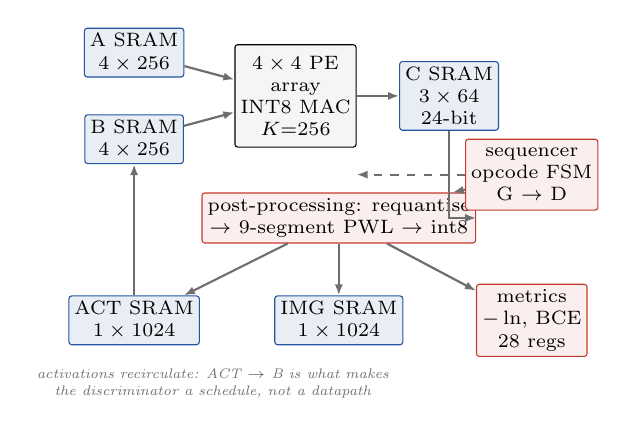
\begin{tikzpicture}[
  font=\scriptsize,
  box/.style={draw,rounded corners=1pt,minimum height=6mm,align=center,inner sep=2pt},
  mem/.style={box,fill=figblue!10,draw=figblue},
  log/.style={box,fill=figred!8,draw=figred},
  ar/.style={-{Latex[length=1.4mm]},figgray,thick}
]
\node[mem,minimum width=11mm] (a) at (0,2.1) {A SRAM\\$4\times256$};
\node[mem,minimum width=11mm] (b) at (0,1.0) {B SRAM\\$4\times256$};
\node[box,fill=black!4,minimum width=14mm,minimum height=13mm] (pe) at (2.05,1.55)
  {$4\times4$ PE\\array\\INT8 MAC\\$K{=}256$};
\node[mem,minimum width=11mm] (c) at (4.0,1.55) {C SRAM\\$3\times64$\\24-bit};
\node[log,minimum width=17mm] (pp) at (2.6,0.0) {post-processing: requantise\\$\rightarrow$ 9-segment PWL $\rightarrow$ int8};
\node[mem,minimum width=12mm] (act) at (0,-1.3) {ACT SRAM\\$1\times1024$};
\node[mem,minimum width=12mm] (img) at (2.6,-1.3) {IMG SRAM\\$1\times1024$};
\node[log,minimum width=12mm] (met) at (5.05,-1.3) {metrics\\$-\ln$, BCE\\28 regs};
\node[log,minimum width=12mm,minimum height=9mm] (seq) at (5.05,0.55) {sequencer\\opcode FSM\\G $\rightarrow$ D};
\draw[ar] (a) -- (pe); \draw[ar] (b) -- (pe); \draw[ar] (pe) -- (c);
\draw[ar] (c) |- (pp); \draw[ar] (pp) -- (act); \draw[ar] (pp) -- (img);
\draw[ar] (pp) -- (met);
\draw[ar] (act) -- (0,0.55) -- (b);
\draw[ar,dashed] (seq) -- (pp); \draw[ar,dashed] (seq) -- (pe.east|-seq);
\node[align=center,font=\tiny\itshape,figgray] at (1.0,-2.1)
  {activations recirculate: ACT $\rightarrow$ B is what makes\\the discriminator a schedule, not a datapath};
\end{tikzpicture}
\caption{The engine. Solid arrows are data, dashed are control. The discriminator adds no block to this figure: it reuses the same array, the same buffers and the same post-processing, differing only in where the sequencer sends results.}
\label{fig:arch}
\end{figure}

\subsection{The discriminator is a schedule, not a datapath}
The natural assumption is that adding a discriminator to a generator accelerator roughly doubles it. It does not. Both networks are dense INT8 layers followed by a bounded activation; they differ in shape, not in kind. In the RTL the entire distinction between a generator layer and a discriminator layer is two values of a destination-select configuration field plus one extra opcode that latches a loss. The MAC array, the operand buffers, the requantiser, the activation unit and the drain paths are shared without modification.

The practical consequence, which we quantify in Section~\ref{sec:mem} and Section~\ref{sec:pins}, is that removing the discriminator to save area would save approximately nothing while costing the forward half of every training step. The same accounting applies at the pins: of the pads this chip uses beyond its predecessor, exactly one is attributable to the discriminator, and even that one is a convenience --- it exposes the verdict bit to an oscilloscope, and the same bit is readable over the serial link.

\subsection{Sequencer}
A single opcode FSM drives the whole adversarial pass: load a weight tile, run the array, flush results through post-processing to a destination, recirculate activations from the activation buffer back into the B operand buffer, score, and latch losses. The host issues opcodes over the serial link; no microcode memory is needed because the opcode set is small and the layer schedule is fixed by configuration registers rather than by instruction sequences.

\section{Piecewise-Linear Activations}\label{sec:pwl}
All six functions the network needs --- tanh, sigmoid, ReLU, LeakyReLU(0.2), identity, and a log$_2$ mantissa used by the loss unit --- share one datapath and one multiplier, selected by a configuration field. Each is a nine-segment piecewise-linear ladder in Q4.12: a comparator chain selects the segment, and one multiply-add evaluates $y = m_ix + c_i$.

Fig.~\ref{fig:pwl} plots the result against the exact functions. Maximum absolute error is 0.04133 for tanh and 0.01966 for sigmoid; the log mantissa fit, which is minimax-fitted rather than inherited, is accurate to 5.16 LSB, and the resulting $-\ln$ used for the cross-entropy losses is accurate to about 0.001 nats.

\begin{figure}[t]
\centering
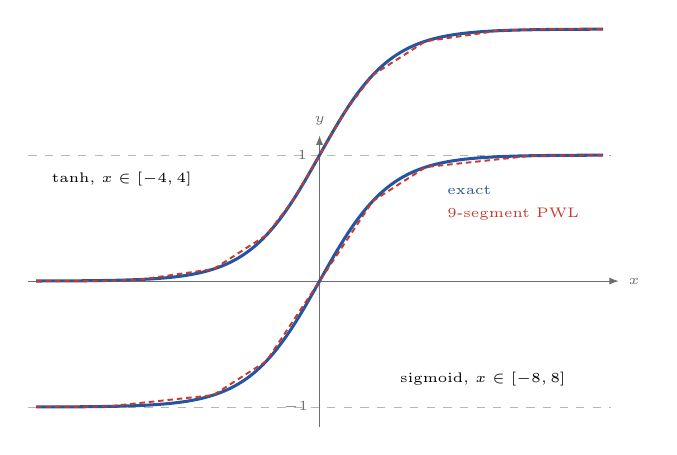
\begin{tikzpicture}[font=\scriptsize]
  \draw[figgray,-{Latex[length=1.2mm]}] (-3.7,0) -- (3.8,0) node[right,font=\tiny] {$x$};
  \draw[figgray,-{Latex[length=1.2mm]}] (0,-1.85) -- (0,1.85) node[above,font=\tiny] {$y$};
  \draw[figgray!50,dashed] (-3.7,1.6) -- (3.7,1.6);
  \draw[figgray!50,dashed] (-3.7,-1.6) -- (3.7,-1.6);
  \node[font=\tiny,figgray] at (-0.22,1.6) {1};
  \node[font=\tiny,figgray] at (-0.3,-1.6) {$-1$};
  \draw[figblue,line width=1.1pt] plot coordinates \tanhexact;
  \draw[figred,line width=0.7pt,dash pattern=on 2pt off 1.4pt] plot coordinates \tanhpwl;
  \draw[figblue,line width=1.1pt] plot coordinates \sigmoidexact;
  \draw[figred,line width=0.7pt,dash pattern=on 2pt off 1.4pt] plot coordinates \sigmoidpwl;
  \node[figblue,font=\tiny,anchor=west] at (1.5,1.15) {exact};
  \node[figred,font=\tiny,anchor=west] at (1.5,0.85) {9-segment PWL};
  \node[font=\tiny,anchor=east] at (-1.5,1.3) {tanh, $x\in[-4,4]$};
  \node[font=\tiny,anchor=west] at (0.9,-1.25) {sigmoid, $x\in[-8,8]$};
\end{tikzpicture}
\caption{Nine-segment approximation against the exact functions, evaluated through the same integer datapath the RTL uses. Curves are drawn on independent horizontal scales; sigmoid is shown over twice the domain of tanh.}
\label{fig:pwl}
\end{figure}

Function-domain error is the wrong metric for a generator, because what matters is the pixel that comes out. Rendering a complete MNIST digit through the approximation and through the 8193-entry table it replaces gives a mean absolute difference of \textbf{1.71 gray levels out of 255}. That is the entire accuracy cost of making the generator implementable.

Two deliberate departures from the reference implementation we ported the coefficients from are worth recording. First, one shared multiplier rather than one per function: the functions are mutually exclusive in time, so the area of five extra multipliers buys nothing. Second, the output is clamped to each function's mathematical range. The reference's outermost sigmoid segments have non-zero slope, so far from the origin it returns values outside $[0,1]$ --- a negative ``probability'' that would corrupt the cross-entropy loss downstream.

\subsection{Folded gain, and why it is exact}
Pre-activations in a Q4.12 word saturate at $\pm 8$, while the real pre-activations of the ReLU layers reach $\pm 180$. Rather than widen the word, a per-layer gain is folded into the requantisation multipliers and undone after the activation. This is exact, not approximate, for the ReLU family because those functions are positively homogeneous: $f(gx) = g\,f(x)$. The tanh and sigmoid layers are not homogeneous and are therefore forced to unit gain --- which costs nothing, because both functions are already flat where the saturation would bite.

\section{Memory Right-Sizing and Batching}\label{sec:mem}
The available SRAM family has a fixed width of 301.3~$\mu$m and scales only in height, so area per stored byte improves steeply with depth: 717, 265, 189 and 152~$\mu$m$^2$ per byte at depths 64, 256, 512 and 1024 respectively. A uniform choice of macro is therefore a poor one. Table~\ref{tab:mem} shows the arrangement adopted.

\begin{table}[t]
\centering
\caption{Operand memory, right-sized across three depths}
\label{tab:mem}
\begin{tabular}{llrr}
\toprule
bank & macros & bytes & area ($\mu$m$^2$) \\
\midrule
A (weights)      & $4\times256\times8$  & 1024 & 271{,}086 \\
B (inputs)       & $4\times256\times8$  & 1024 & 271{,}086 \\
C (accumulators) & $3\times64\times8$   & 192  & 137{,}583 \\
ACT (activations)& $1\times1024\times8$ & 1024 & 155{,}414 \\
IMG (image)      & $1\times1024\times8$ & 1024 & 155{,}414 \\
\midrule
total            & 13 macros            & 4288 & \textbf{990{,}581} \\
prior uniform    & $16\times256\times8$ & 4096 & 1{,}084{,}343 \\
\bottomrule
\end{tabular}
\end{table}

The result is 8.6\% less macro area than the uniform arrangement, with 91\% bank utilisation, while simultaneously enabling four-way batching. A and B need four parallel byte lanes and cannot be merged --- A holds four weight rows, B four batch columns --- but C never holds more than $N^2 = 16$ words, so 256-deep macros there wasted 94\% of their depth, and the two new buffers want depth rather than width.

Batching follows from the array's shape. The $4\times4$ array was always a matrix--matrix engine: B's four columns can hold four independent input vectors, and C's sixteen words are then four neurons across four lanes. One streamed weight tile therefore serves four images. Because weight streaming dominates run time --- a matrix--vector product has no weight reuse whatsoever, at 1.01 weight bytes per MAC --- this is close to a linear win: \textbf{103{,}398 compute cycles per digit at batch~4 against 440{,}252 at batch~1, a $4.26\times$ improvement}, verified end to end with all four lanes bit-exact. Four full images do not fit on chip, so the host holds them and the image buffer becomes a drain window; the accuracy cost of sharing one calibration across four latents is 0.15--0.59 gray levels.

\section{Host Link}\label{sec:link}
The chip talks to its host over four wires. In the base protocol every byte costs a 24-edge frame, which makes the link, not the array, the entire latency of the system. Two burst commands remove that. \texttt{WR\_BURST} sends the start address once and auto-increments, costing 8 edges per byte; \texttt{WR\_BURST8} additionally takes the byte off an 8-bit parallel bus, costing one edge per byte. Measured at the pads over a full 1024-byte tile:

\begin{table}[t]
\centering
\caption{Measured host-link cost for one 1024-byte weight tile}
\label{tab:link}
\begin{tabular}{lrrr}
\toprule
mode & SCLK edges & per byte & speed-up \\
\midrule
single-byte frames & 24{,}576 & 24.00 & $1.00\times$ \\
serial burst       &  8{,}208 &  8.01 & $2.99\times$ \\
parallel burst     &  1{,}040 &  1.01 & $23.63\times$ \\
\bottomrule
\end{tabular}
\end{table}

Counting every host write, including the discriminator's 784-wide input which must be re-fed per weight tile at batch~4, the two mechanisms together take end-to-end latency from \textbf{9.45~s to 0.161~s per image}, a $58.5\times$ improvement. The $4.26\times$ compute figure is separate from and unaffected by this.

The parallel bus is only worth its eight pads if the host can write a byte in one register store, which requires allocating those pads to eight contiguous bits of one GPIO port. Scattered across ports, the host spends eight bit-bang writes per byte and the advantage is gone.

\section{Pins}\label{sec:pins}
The engine's internal interface is 106 signal bits, and the target shuttle slot offers 20 general-purpose digital pads. Serialisation absorbs the difference: 17 pads are used --- four for the link, four for status, eight for the parallel burst bus, and one mirroring the readback line so that a single failed bond cannot blind the chip --- and three remain spare. Minimum viable bring-up needs seven signals plus one supply rail: clock, reset, the four link wires, and a busy flag. Opcodes are not pins; they travel inside the address field of the link frame, which is why the command set can grow without touching the pad budget.

\section{Host-in-the-Loop Training}
Because every activation on this chip has a derivative expressible in terms of its own \emph{output} --- $\mathrm{ReLU}' = [a>0]$, $\tanh' = 1-a^2$, $\sigma' = a(1-a)$ --- and because those outputs already drain over the existing read commands, host-side backpropagation needs no new hardware. The chip performs the forward pass of both networks; the host keeps float master weights, recalibrates per step, and applies the optimiser. A driver closes this loop and is bit-exact against the golden model. The cost is roughly 20\% additional link traffic for the drains, which a burst \emph{read} command would largely remove --- the one addition to this design we would recommend making before silicon.

\section{Physical Implementation}\label{sec:phys}
The engine hardens as a single macro on a $1900\times1900~\mu$m die with all 13 SRAM macros placed, using the same native-3.3~V standard-cell library and single-supply operating point as the prior chip. Table~\ref{tab:signoff} reports the sign-off.

\begin{table}[t]
\centering
\caption{Sign-off of the hardened engine macro}
\label{tab:signoff}
\begin{tabular}{ll}
\toprule
metric & value \\
\midrule
die / macros            & $1900\times1900~\mu$m, 13 SRAM \\
clock                   & 40~ns (25~MHz), 9 corners \\
setup / hold worst slack& $+12.30$~ns / $+0.118$~ns \\
Magic DRC / LVS / XOR   & 0 / 0 / 0 \\
routing DRC             & 0 \\
antenna nets / pins     & \textbf{0 / 0} \\
power (typical)         & 228~mW \\
reproducibility         & byte-identical placement DB \\
\bottomrule
\end{tabular}
\end{table}

\begin{figure}[t]
\centering
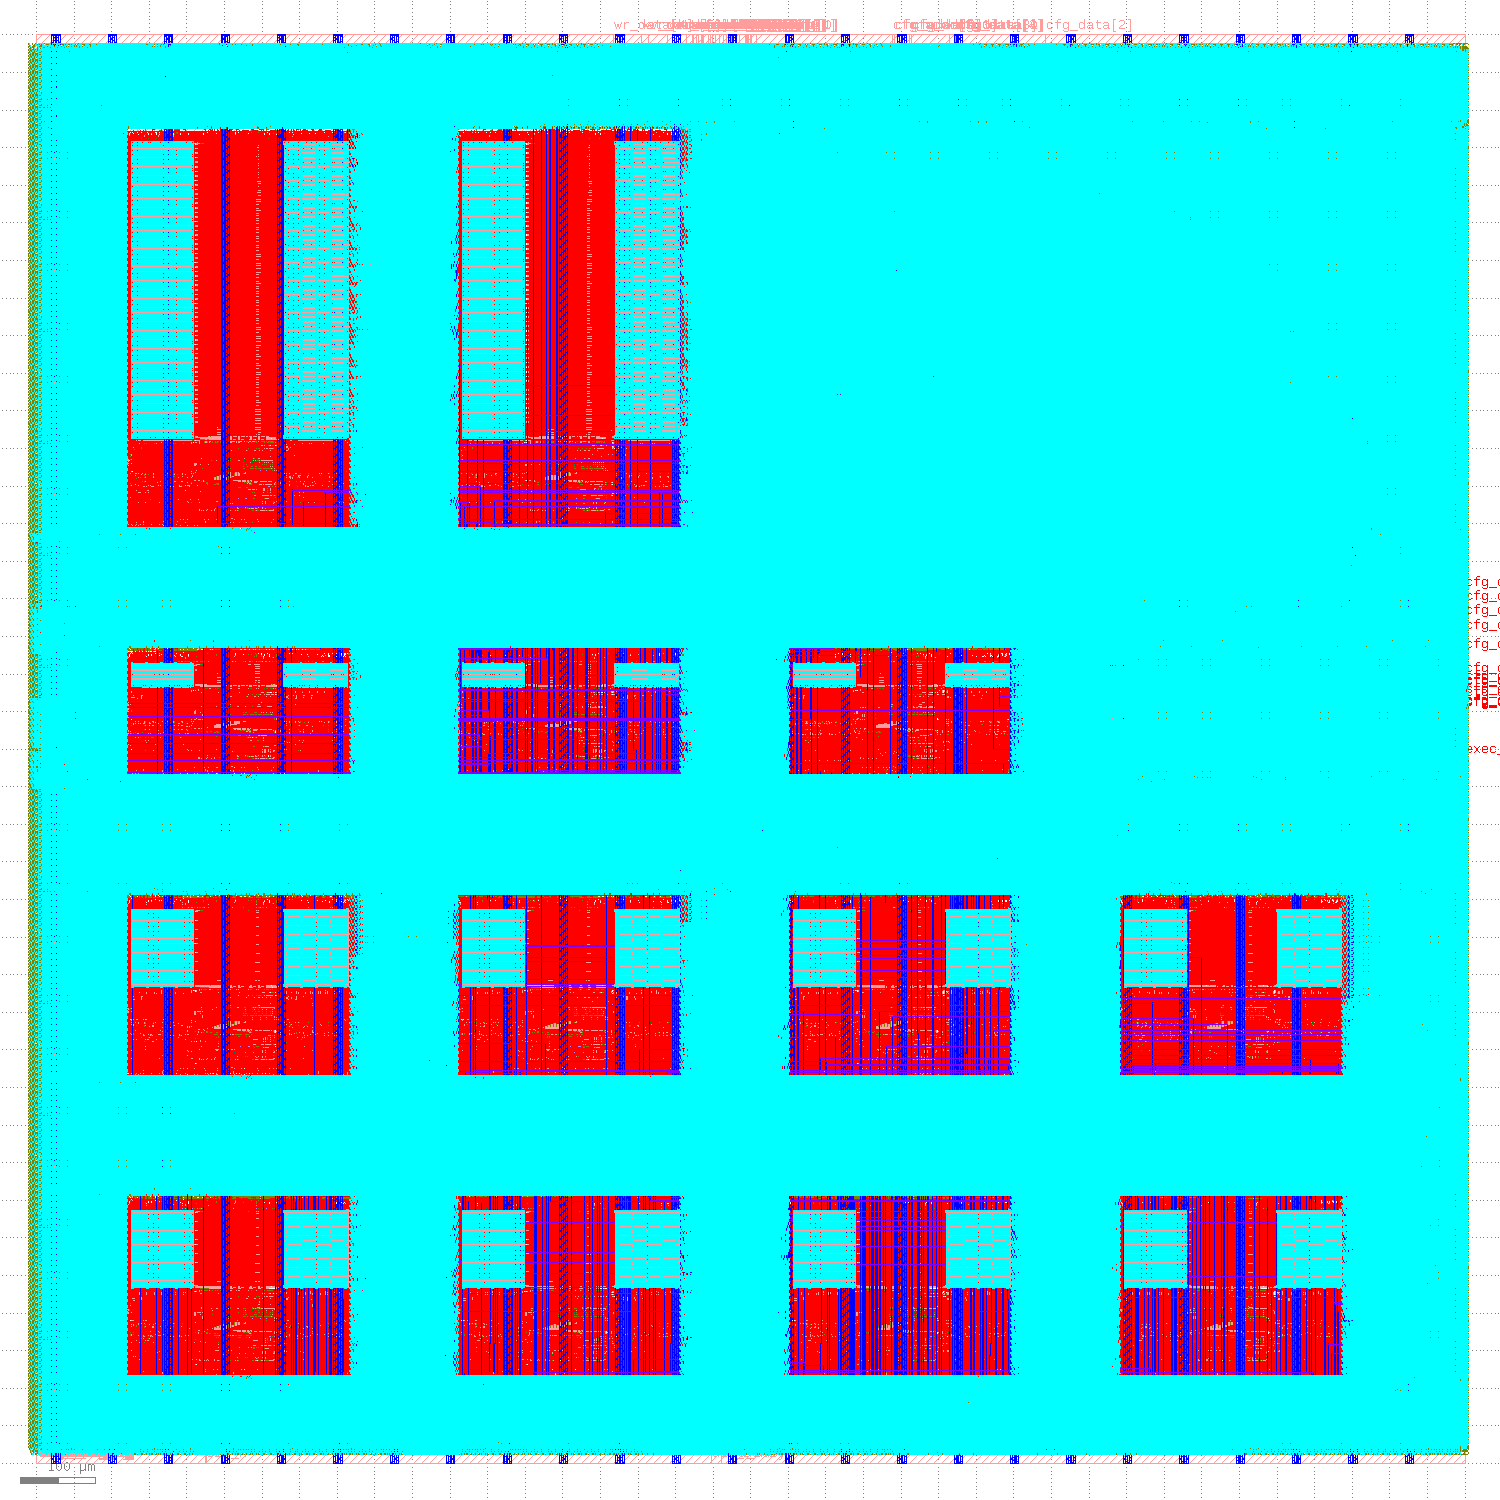
\includegraphics[width=0.80\columnwidth]{gan_macro_gds.png}
\caption{The hardened engine macro, $1900\times1900~\mu$m. The right-sized memory is visible as three distinct macro heights: the two 1024-deep buffers at the top, the three 64-deep accumulator byte-planes in the middle, and the eight 256-deep operand macros below.}
\label{fig:gds}
\end{figure}

The clock was set by measurement rather than estimate. The first routed run closed a deliberately conservative 60~ns target with $+27.56$~ns of slack, i.e.\ a real critical path of 32.44~ns, which showed that the $28\times20$ array multiplier added by post-processing was not the bottleneck it had been sized for. Retiming to 40~ns matched the prior chip exactly and scaled power by precisely $1.5\times$, identifying the macro as dynamic-power dominated.

\subsection{A correction on antenna closure}
Antenna violations on this process are a per-net, per-layer metal-area rule, non-gating in this flow but worth closing as a quality goal. Our prior work closed them by perturbing the placement density, and we reported that lever as behaving like a re-roll rather than an optimisation.

On this design the same lever initially appeared exhausted. Sampling densities 58 through 63 gave counts of 3, 2, 2, 6, 5 and 12, a floor of two reached from both sides, and the survivors were not marginal: each was a $>2.7\times$ violation on a long broadcast net between an SRAM macro and the array. We concluded in an earlier draft of this work that the cause was structural and that only a floorplan change could fix it.

That conclusion was wrong, and Fig.~\ref{fig:sweep} shows why. Every sample had been taken at or above the starting point of 60. Extending the sweep \emph{downward} not only reduces the count but changes the kind of violation: structural at 59--60, all-marginal at 57--58, and none at all at 56.

\begin{figure}[t]
\centering
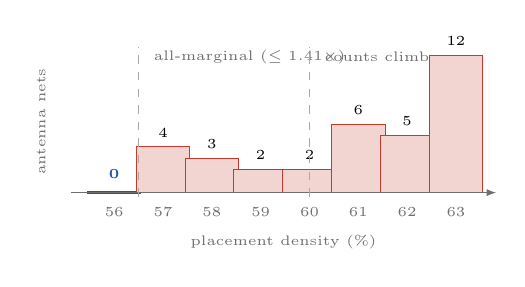
\begin{tikzpicture}[font=\scriptsize]
\def\bw{0.34}
\foreach \d/\n/\i in {56/0/0, 57/4/1, 58/3/2, 59/2/3, 60/2/4, 61/6/5, 62/5/6, 63/12/7} {
  \pgfmathsetmacro\x{\i*0.62}
  \pgfmathsetmacro\h{\n*0.145}
  \ifnum\n=0
    \draw[figblue,line width=0.9pt] (\x-\bw,0) -- (\x+\bw,0);
    \node[figblue,font=\tiny\bfseries,anchor=south] at (\x,0.06) {0};
  \else
    \filldraw[fill=figred!22,draw=figred] (\x-\bw,0) rectangle (\x+\bw,\h);
    \node[font=\tiny,anchor=south] at (\x,\h) {\n};
  \fi
  \node[font=\tiny,anchor=north,figgray] at (\x,-0.06) {\d};
}
\draw[figgray,-{Latex[length=1.2mm]}] (-0.55,0) -- (4.85,0);
\node[font=\tiny,figgray,anchor=north] at (2.15,-0.42) {placement density (\%)};
\node[font=\tiny,figgray,rotate=90,anchor=south] at (-0.75,0.9) {antenna nets};
\draw[figgray!60,dashed] (0.31,-0.05) -- (0.31,1.85);
\node[font=\tiny,anchor=west,figgray] at (0.38,1.72) {all-marginal ($\le 1.41\times$)};
\draw[figgray!60,dashed] (2.48,-0.05) -- (2.48,1.85);
\node[font=\tiny,anchor=west,figgray] at (2.55,1.72) {counts climb};
\end{tikzpicture}
\caption{The full sweep. The earlier conclusion was drawn from the samples at 58 and above; the value that closes is below all of them.}
\label{fig:sweep}
\end{figure}

The mechanism in the original reading was right --- the $>2.7\times$ nets really are long macro-to-array broadcasts, and they really do not move anywhere between 59 and 63. What was wrong was the inference from ``this lever cannot shift these nets'' to ``no value of this lever can''. A looser placement leaves the router room to detour a long net; a tighter one takes it away, which is why the counts climb steeply above 60. We state the correction explicitly because the failure mode is easy to repeat: a lever sampled on only one side of its starting point can look exhausted when it has not been explored. The result is reproducible in the strong sense --- re-running the promoted configuration produces a byte-identical placement database.

Should the problem recur after a netlist change, the evidence points at a more targeted lever than either density or floorplan: every violation across all ten routed runs of this design was on the same metal layer, so reducing that layer's routing capacity should push the long nets upward, where the upper layer is nearly empty.

\subsection{What changed relative to the prior chip}
Table~\ref{tab:cmp} summarises the difference. The engine grew from a matrix-multiply
accelerator into a complete adversarial pipeline, and the die grew with it, but the
external interface did not: the same shuttle slot, the same two dedicated pads, the same
single supply, and three spare general-purpose pads left over.

\begin{table}[t]
\centering
\caption{This work against the prior accelerator}
\label{tab:cmp}
\begin{tabular}{lll}
\toprule
 & prior~\cite{apic_a} & this work \\
\midrule
on chip        & generator MACs & G + D, losses, metrics \\
activations    & testbench LUT  & 9-segment PWL, on die \\
SRAM macros    & 11 ($\times256$) & 13 (64/256/1024) \\
buffer bytes   & 2816 & 4288 \\
batch lanes    & 1 & 4 \\
engine die     & $1600\times1500~\mu$m & $1900\times1900~\mu$m \\
clock          & 40~ns & 40~ns \\
antenna        & 0 / 0 & 0 / 0 \\
digital pads   & 7 of 20 & 17 of 20 \\
end-to-end     & 1.61~s/image & 0.161~s/image \\
\bottomrule
\end{tabular}
\end{table}

\subsection{Chip-level integration}\label{sec:chiplevel}
The macro is then placed inside the shuttle padring, behind the serial bridge, and the
complete chip is taken through the same flow. One template setting had to change. The
padring's own configuration enables the detailed router's in-place antenna repair, which
on this chip aborts routing with a no-access-point error on a diode the repair itself had
just placed --- the same wall this project documented from five directions on the engine
macro, where any non-zero repair iteration count triggers a verification re-route whose
pin-access phase must reach diodes that have none. The prior, smaller chip survived the
same setting; this one, with roughly twice the glue logic and more pre-route violations,
does not. Disabling that repair lets routing complete.

\section{Verification}
Correctness is checked against a single Python golden model at every level. The activation and loss units match over 1858 directed vectors. A full adversarial pass matches bit-exactly on all 784 pixels plus both scores, both losses and every metric register. The four-way batched flow matches on \textbf{3136 of 3136 pixels} across four lanes simultaneously, with the four scores distinct and the replicated real-image scores identical --- a lane-crossing bug would break that symmetry. The pad-level testbench drives the physical pins rather than internal ports and reproduces the measured burst edge counts of Table~\ref{tab:link}. The prior chip's own regression suite passes unchanged.

\section{Discussion and Limitations}
Three limitations are worth stating plainly. The loss registers saturate at 8.32 nats, because a Q4.12 probability cannot represent $y < 2^{-12}$; this affects only the reported metric, not the computation. The activation approximation costs 1.71 gray levels, which is invisible in a rendered digit but is not zero. And the shared calibration across a batch costs a further 0.15--0.59 gray levels, which is the price of the $4.26\times$.

The broader observation from this work is about where the boundary between hardware and software actually falls in a small generative model. The discriminator, which sounds like a second accelerator, is a schedule. The training loop, which sounds like it needs dedicated gradient hardware, needs none, because every activation's derivative is a function of its own output and those outputs already leave the chip. What genuinely had to become hardware was the least glamorous part: a nine-segment approximation to two curves.

\section{Conclusion}
A complete GAN --- generator, discriminator, bounded activations, both cross-entropy losses and their metrics --- fits on an open-PDK 180~nm die behind an unchanged pin budget, and hardens with zero DRC, LVS and antenna violations at 40~ns on a single 3.3~V supply. Right-sizing the operand memory across three depths made the design 8.6\% smaller while paying for $4.26\times$ batching, and burst commands on the host link took end-to-end latency from 9.45~s to 0.161~s per image. The parts that were hard were not the parts that sound hard.

\section*{Acknowledgment}
The authors thank the open-source EDA community, the GlobalFoundries open PDK program for GF180MCU and its SRAM macros, and the wafer.space chipathon program for the padring template and shuttle slot targeted by this work.

\begin{thebibliography}{9}
\bibitem{apic_a} W. Anthony, I M. M. Surya W.M., J. R. Saragi, M. P. Adipratama, and F. A. Rahagi, ``An 8-bit deep learning accelerator for GAN image generation on GF180MCU,'' in \emph{Proc. APSIPA ASC}, 2026.
\bibitem{gf180} GlobalFoundries and Google, ``GF180MCU open process design kit,'' 2022. [Online]. Available: \url{https://github.com/google/gf180mcu-pdk}
\bibitem{librelane} LibreLane Contributors, ``LibreLane: an open-source RTL-to-GDSII flow,'' 2025. [Online]. Available: \url{https://github.com/librelane/librelane}
\bibitem{openroad} T. Ajayi \emph{et al.}, ``OpenROAD: toward a self-driving, open-source digital layout implementation tool chain,'' in \emph{Proc. GOMACTech}, 2019.
\bibitem{goodfellow} I. Goodfellow \emph{et al.}, ``Generative adversarial nets,'' in \emph{Adv. Neural Inf. Process. Syst.}, 2014.
\bibitem{jacob} B. Jacob \emph{et al.}, ``Quantization and training of neural networks for efficient integer-arithmetic-only inference,'' in \emph{Proc. IEEE CVPR}, 2018.
\end{thebibliography}

\end{document}
